% !TEX encoding = UTF-8 Unicode
\documentclass[accentcolor=tud6b,colorbacktitle,inverttitle,landscape,german,presentation,t]{tudbeamer}
\usepackage{ngerman}
\usepackage[utf8]{inputenc}
\usepackage{graphicx}
\providecommand\thispdfpagelabel[1]{}

\begin{document}

\title[MLDM: Projekt Aufgabe 1-3]{Maschinelles Lernen Symbolische Ansätze:\\ Projekt Aufgaben 1-3}
\subtitle{}

\author[bremer\_endreß\_fahrer]{Joachim Bremer, Jeannine Endreß, Uli Fahrer}
%\institute[]{}

\date{\today}

\begin{titleframe}
\tableofcontents
\end{titleframe}

    \section{Aufgabe 1 - Regellernen: Anwendung und Interpretation}
    
    \subsection{Verwendete Datensätze und Regellerner}
    
    \begin{frame}[t]
    \frametitle{Aufgabe 1 - Regellernen: Anwendung und Interpretation\\ Verwendete Datensätze und Regellerner}
        \begin{itemize}
            \item Car Evaluation Database
            \item Database for Fitting Contact Lenses
            \item Zoo Database
            \begin{itemize}
                \item Attribut 14 ist numerisch (Anzahl der Beine)
                \item Preprocessing mit Unsupervized Discretiser nötig
                \item Liefert fünf Bins (Intervalle) für 0, 2, 4, 6 oder 8 Beine
            \end{itemize}
        \end{itemize}
        \vfill
        $\rightarrow$ Klassifizieren mit ConjunctiveRule, JRip und Prism\\
        $\rightarrow$ Test mit training set als Testoption //TODO!!!
    \end{frame}
    
    \subsection{Vergleich der Ergebnisse: Datensätze}
    
    \begin{frame}[t]
    \frametitle{Aufgabe 1 - Regellernen: Anwendung und Interpretation\\ Vergleich der Ergebnisse: Datensätze}
        Car Datensatz (4 Klassen):
      
        \begin{itemize}
            \item ConjunctiveRule: produziert (\texttt{true $\Rightarrow$ class=unacc}) als einzige, bedingungslose Regel            
            \begin{itemize}
                \item Es wird immer nur eine Klasse vorhergesagt.
            \end{itemize}
            \item JRip: 49 Regeln mit durchschnittlich 4 Bedingungen 
            \begin{itemize}
                \item Im Mittel: Vorhersage aller Klassen mit 88\% Precision und 87\% Recall
            \end{itemize}
            \item Prism: deutlich mehr Regeln und eine etwas bessere Accuracy als JRip 
            \begin{itemize}
                \item  Aber evtl. Overfitting da sehr viele Bedingungen pro Regel
            \end{itemize}
        \end{itemize}
    \end{frame}
    
     \begin{frame}[t]
    \frametitle{Aufgabe 1 - Regellernen: Anwendung und Interpretation\\ Vergleich der Ergebnisse: Datensätze}
        Contact Lenses Datensatz (3 Klassen):
        \begin{itemize}
            \item ConjunctiveRule: produziert mit (\texttt{true $\Rightarrow$ contact-lenses=none}) eine bedingungslose Regel
            \begin{itemize}
                \item Es wird nur die häufigste Klasse vorhergesagt (höchster Prior).
            \end{itemize}
            \item JRip: 3 Regeln mit 0, 1 oder 2 Bedingungen um alle 3 Klassen vorherzusagen
            \item Prism: Mehr und spezifischere Regeln 
            \begin{itemize}
                \item Teilweise alle 4 Attribute als Bedingung
                \item Schlechtere Accuracy als JRip
            \end{itemize}
        \end{itemize}
    \end{frame}
    
    \begin{frame}[t]
    \frametitle{Aufgabe 1 - Regellernen: Anwendung und Interpretation\\ Vergleich der Ergebnisse: Datensätze}
        Zoo Datensatz (7 Klassen):
        \begin{itemize}
            \item ConjunctiveRule: produziert (\texttt{milk=true $\Rightarrow$ type=mammal}) als einzige Regel mit einer Bedingung
            \begin{itemize}
                \item Deshalb werden nicht alle Klassen vorhergesagt.
            \end{itemize}
            \item JRip: 7 Regeln mit maximal 3 Bedingungen
             \begin{itemize}
                \item  Accuracy von 89\% für alle Klassen zusammen
            \end{itemize}
            \item Prism: Deutlich speziellere Regeln 
            \begin{itemize}
               \item Für die meisten Tiernamen direkt den Typ gelernt $\rightarrow$ fast keine Generalisierung!
                \item Im Vergleich zu JRip: weniger Beispiele korrekt klassifiziert
            \end{itemize}
        \end{itemize}
    \end{frame}    
   
    
    \subsection{Vergleich der Ergebnisse: Regellerner}
    
    \begin{frame}[t]
    \frametitle{Aufgabe 1 - Regellernen: Anwendung und Interpretation\\ Vergleich der Ergebnisse: Regellerner}
        ConjunctiveRule:
        \begin{itemize}
            \item Es wird immer genau eine Regel gelernt.
            \begin{itemize}
                \item  Die Regel, die häufigste Klasse vorhersagt!
            \end{itemize}
            \item In 2 Fällen entspricht die Regel dem höchsten Prior, da sie keine Bedingung hat.
            \item Beim Zoo Datensatz wird für Beispiele, bei denen die Bedingung \texttt{milk=true $\Rightarrow$ type=mammal} nicht erfüllt ist,
                  als Default-Value die nächst häufigste Klasse \texttt{bird} zugewiesen
        \end{itemize}
    \end{frame}
    
    \begin{frame}[t]
    \frametitle{Aufgabe 1 - Regellernen: Anwendung und Interpretation\\ Vergleich der Ergebnisse: Regellerner}
        JRip:
        \begin{itemize}
            \item Vergleichsweise werden wenige generelle Regeln gelernt.
            \item Passt zur \texttt{Information Gain} Heuristik, da diese allgemeinere Regeln bevorzugt
            \item Die Default-Rule wählt die häufigste Klasse aus, wenn keine andere Regel davor zutrifft
            \begin{itemize}
                \item Prinzip: ``Wenn kein weiteres Wissen vorhanden ist, dann wähle die Klasse, die am meisten vorkommt.''
            \end{itemize}
        \end{itemize}
    \end{frame}
    
    \begin{frame}[t]
    \frametitle{Aufgabe 1 - Regellernen: Anwendung und Interpretation\\ Vergleich der Ergebnisse: Regellerner}
        Prism:
        \begin{itemize}
            \item Vergleichsweise werden viele spezielle Regeln gelernt.
            \item Passt zur \texttt{Precision} Heuristik, die zu Overfitting neigt.
            \item Es gibt keine Default-Rule.
        \end{itemize}
    \end{frame}
    
    \subsection{Zusammenfassung}    
    \begin{frame}[t]
    \frametitle{Aufgabe 1 - Regellernen: Anwendung und Interpretation\\ Zusammenfassung}
        \begin{itemize}
            \item Insgesamt lernt JRip die Datenmengen am Besten.
            \item Das Ergebnis passt zur benutzten Heuristik, die allgemeinere Regeln bevorzugt und Overfitting vermeidet.
            \item Außerdem lässt sich der Car-Datensatz am genauesten Lernen 
            \begin{itemize}
                \item (Vermutlich, weil er am Größten ist und dadurch viele Beispiele zum Lernen existieren
            \end{itemize}
            \item Für fundiertere Aussagen sind weitere Untersuchungen mit größeren Datensätzen notwendig, da insgesamt eine große Abhängigkeit von den jeweiligen Daten zu beobachten ist.
        \end{itemize}
    \end{frame}
    
    \section{Aufgabe 2 - Evaluation von Regellernern}
    
    \subsection{Verwendete Datensätze}
    
    \begin{frame}[t]
    \frametitle{Aufgabe 2 - Evaluation von Regellernern\\ Verwendete Datensätze}
        \begin{itemize}
            \item Balance Scale Weight \& Distance Database
            \item Car Evaluation Database
            \item Thyroid Disease Records (``Sick'' Datensatz)
            \item Sonar: Mines vs. Rocks
            \item 1984 United States Congressional Voting Records Database
        \end{itemize}
        \vfill
        $\rightarrow$ Datensätze jeweils zufällig mischen und dann in 2 gleich große Teile aufteilen\\
        $\rightarrow$ Danach mit JRip auf Trainingsdatensatz lernen und evaluieren
    \end{frame}
    
    \subsection{Vergleich Verschiedener Validierungsmethoden}
    
    \begin{frame}[t]
    \frametitle{Aufgabe 2 - Evaluation von Regellernern\\ Vergleich Verschiedener Validierungsmethoden}
        Resultierende Genauigkeitsabschätzungen:
        \vfill
        \begin{tabular}[htbp]{l||c|c|c|c|c}
            Datensatz & 1x5 CV & 1x10 CV & 1x20 CV & Leave-One-Out & Trainingsmenge \\
            \hline
            \hline
            Balance & 78.2051 & 80.1282 & 75.641 & 78.2051 & 83.0128 \\
            \hline
            Car & 77.4306 & 79.8611 & 80.2083 & 79.2824 & 87.5 \\
            \hline
            Sick & 98.0382 & 97.9852 & 98.1972 & 98.3563 & 99.0456 \\
            \hline
            Sonar & 75.9615 & 75 & 75 & 73.0769 & 94.2308 \\
            \hline
            Vote & 94.0367 & 95.4128 & 93.578 & 95.4128 & 95.4128 \\
        \end{tabular}
        \vfill
        $\rightarrow$ Definitiv ist Testen auf der Trainingsmenge nicht empfehlenswert, da die Accuracy des gelernten Modells überschätzt wird (Overfitting)\\
        $\rightarrow$ Die verschiedenen Cross-Validation Ergebnisse liefern bis jetzt kein aussagekräftiges Muster bzgl. ihrer Qualität (weitere Untersuchung nötig)
    \end{frame}
    
    \subsection{Unterschiedliche Random Seeds für 10x10 Cross-Validation}
    
    \begin{frame}[t]
    \frametitle{Aufgabe 2 - Evaluation von Regellernern\\ Unterschiedliche Random Seeds für 10x10 Cross-Validation}
        Vergleich 1x10 vs. 10x10 Cross-Validation
        \vfill
        \begin{tabular}[htbp]{l||c|c}
            Datensatz & 1x10 CV & 10x10 CV \\
            \hline
            \hline
            Balance & 80.1282 & 77.82052 \\
            \hline
            Car & 79.8611 & 79.71065 \\
            \hline
            Sick & 97.9852 & 98.27148 \\
            \hline
            Sonar & 75 & 73.36538 \\
            \hline
            Vote & 95.4128 & 94.9541 \\
        \end{tabular}
        \vfill
        Gemittelte Genauigkeiten der 10 verschiedenen Durchläufe weichen nicht allzu stark vom Ursprungsergebnis ab.\\
        Aber während der Berechnung ist aufgefallen, dass je nach Random Seed Schwankungen von $\pm 4\%$ zwischen den einzelnen 1x10 CVs auftreten.\\
        $\rightarrow$ Für robustere Aussagen sind also mehrere Läufe mit jeweils neuer Random Initialisierung sinnvoll
    \end{frame}
    
    \subsection{Genauigkeitsmessung auf Testdatensatz}
    
    \begin{frame}[t]
    \frametitle{Aufgabe 2 - Evaluation von Regellernern\\ Genauigkeitsmessung auf Testdatensatz}
        Vergleich 10x10 Cross-Validation vs. Validierungsmenge
        \vfill
        \begin{tabular}[htbp]{l||c|c}
            Datensatz & 10x10 CV & Testmenge \\
            \hline
            \hline
            Balance & 77.82052 & 78.2748 \\
            \hline
            Car & 79.71065 & 81.9444 \\
            \hline
            Sick & 98.27148 & 98.0382 \\
            \hline
            Sonar & 73.36538 & 67.3077 \\
            \hline
            Vote & 94.9541 & 95.8525 \\
        \end{tabular}
        \vfill
        Evaluation des gelernten Modells auf Testdaten liefert meistens eine Accuracy der selben Größenordnung.
        In einem Fall ist die Abschätzung aber auffallend niedriger.\\
        $\rightarrow$ Für eine realistischere Validierung ist es sinnvoll, mit ungesehenen Testdaten zu evaluieren (bessere Überprüfung der Generalisierbarkeit)
    \end{frame}
    
    \section{Aufgabe 3 - ROC-Kurven}
    
    \subsection{Klassifikationsdatensatz}
    
    \begin{frame}[t]
    \frametitle{Aufgabe 3 - ROC-Kurven\\ Klassifikationsdatensatz}
        \vfill
        \begin{itemize}
            \item Datensatz ``Vote'' jeweils mit J48 und NaiveBayes klassifiziert
            \item Anschließend jeweils beide ROC-Kurven für die Klassen ``republicans'' und ``democrats'' generiert
        \end{itemize}
    \end{frame}
    
    \subsection{Vergleich der Erzeugten Kurven}
    
    \begin{frame}[t]
    \frametitle{Aufgabe 3 - ROC-Kurven\\ Vergleich der Erzeugten Kurven}
        \begin{figure}[htbp]
            \centering
            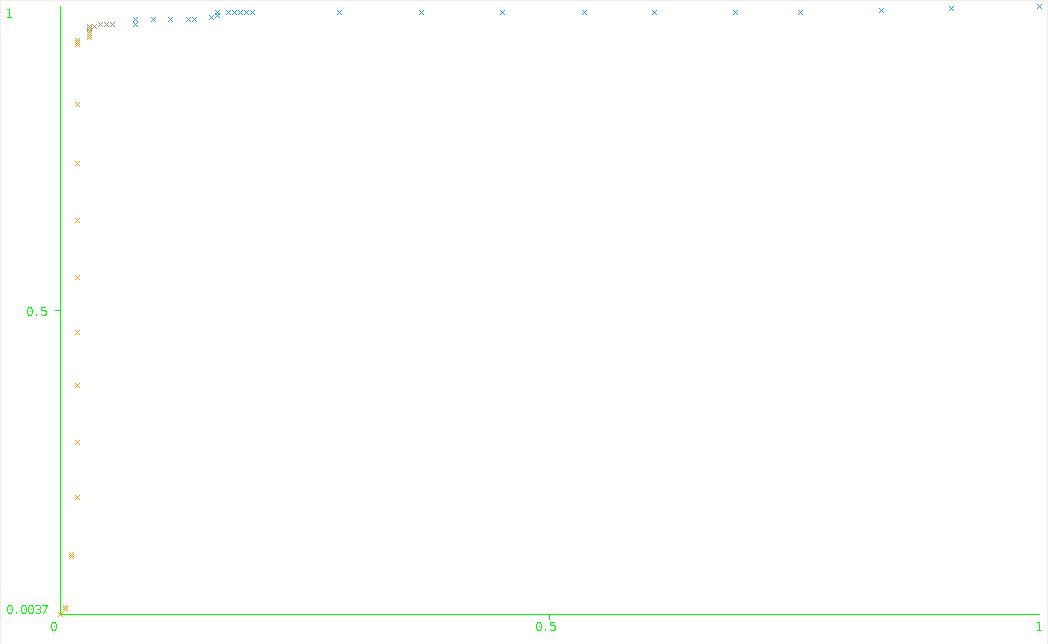
\includegraphics[height=5cm]{roc-j48-democrats}
            \caption{J48 - ROC-Kurve für die Klasse ``democrats''}
        \end{figure}
    \end{frame}
    
    \begin{frame}[t]
    \frametitle{Aufgabe 3 - ROC-Kurven\\ Vergleich der Erzeugten Kurven}
        \begin{figure}[htbp]
            \centering
            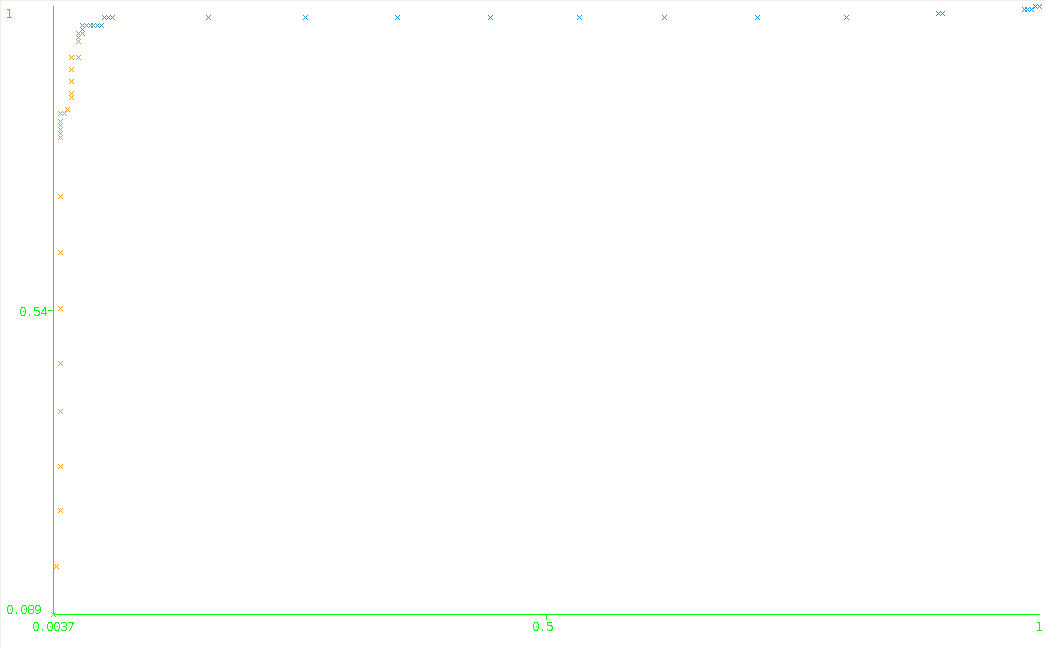
\includegraphics[height=5cm]{roc-j48-republicans}
            \caption{J48 - ROC-Kurve für die Klasse ``republicans''}
        \end{figure}
    \end{frame}
    
    \begin{frame}[t]
    \frametitle{Aufgabe 3 - ROC-Kurven\\ Vergleich der Erzeugten Kurven}
        \begin{figure}[htbp]
            \centering
            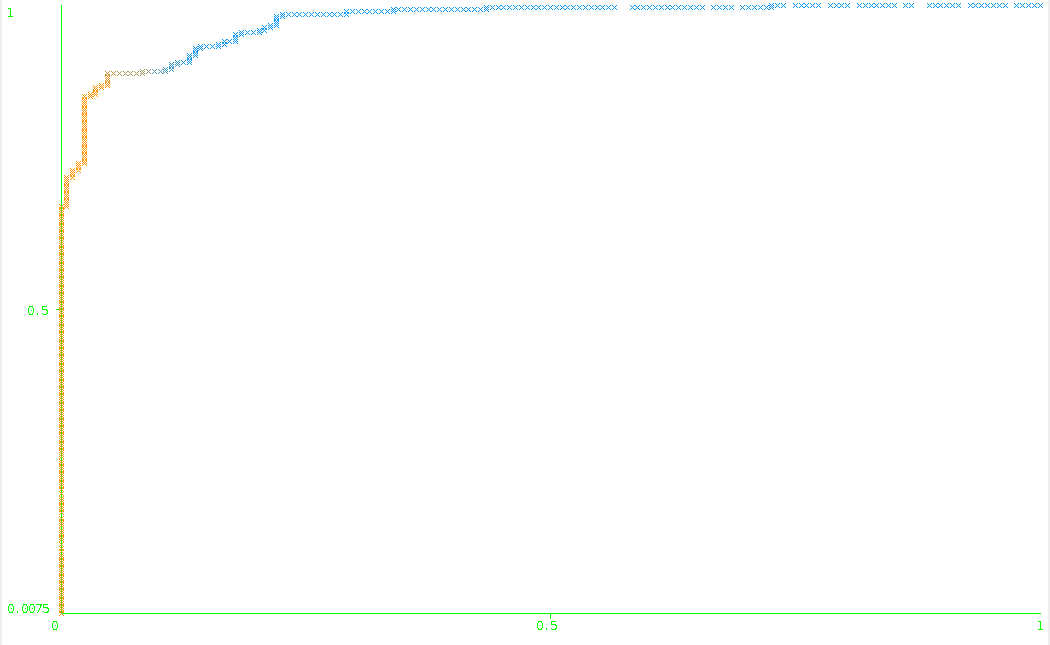
\includegraphics[height=5cm]{roc-naivebayes-democrats}
            \caption{NaiveBayes - ROC-Kurve für die Klasse ``democrats''}
        \end{figure}
    \end{frame}
    
    \begin{frame}[t]
    \frametitle{Aufgabe 3 - ROC-Kurven\\ Vergleich der Erzeugten Kurven}
        \begin{figure}[htbp]
            \centering
            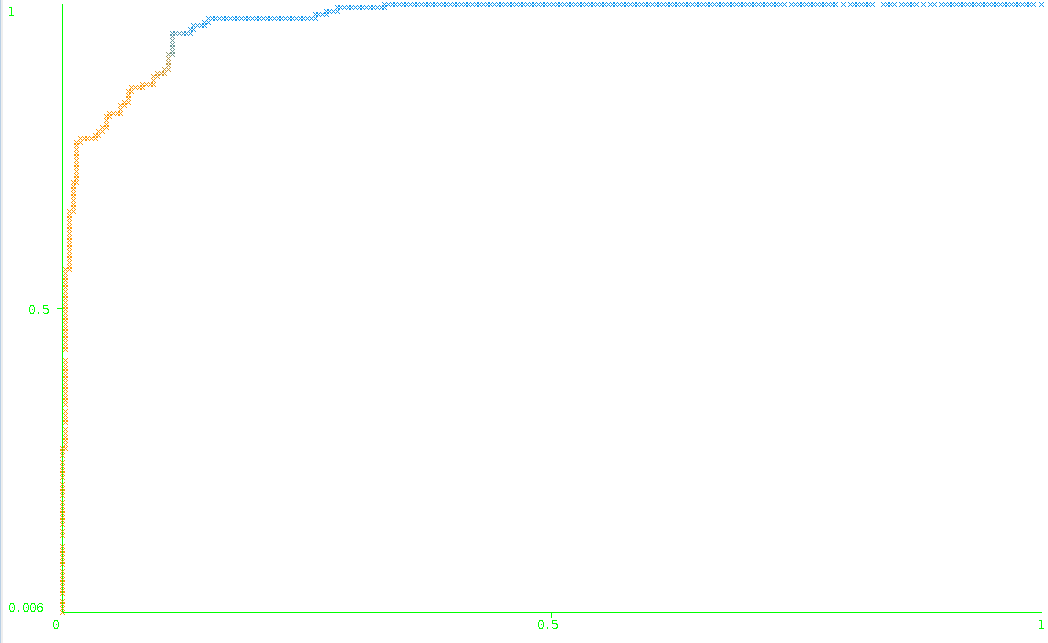
\includegraphics[height=5cm]{roc-naivebayes-republicans}
            \caption{NaiveBayes - ROC-Kurve für die Klasse ``republicans''}
        \end{figure}
    \end{frame}
    
    \subsection{Interpretation der Resultate}
    
    \begin{frame}[t]
    \frametitle{Aufgabe 3 - ROC-Kurven\\ Interpretation der Resultate}
        Zunächst einmal fällt auf dass die Kurven sehr konvex sind\\
        $\rightarrow$ Gute Trennung der Klassen
        \vfill 
        Die ROC-Kurven für J48 nähern sich am meisten dem Punkt der optimalen Theorie an (true-positive-rate 100\% und false-positive-rate 0\%).\\
        Die ``Area Under ROC'' von J48 hüllt diejenige von NaiveBayes fast in ihrer Gesamtheit ein.
        \vfill
        $\rightarrow$ Für diesen Datensatz scheint J48 also nahezu immer ein besserer Klassifizierer als NaiveBayes zu sein\\
        $\rightarrow$ Nur für sehr steile Kostenverhältnisse (fpr minimal, sehr hohe Precision) bzw. für sehr flache Kostenverhältnisse (tpr maximal, sehr hoher Recall) kann NaiveBayes sinnvoll sein
    \end{frame}

\begin{frame}
\frametitle{Abschlussüberblick}
\tableofcontents
\begin{center}
\textbf{\Large FRAGEN?}
\end{center}
\end{frame}

\begin{frame}
\frametitle{Gruppenmitglieder}
Matthias Krebs, 1620340 \vfill
Thomas Pignede, 1626386 \vfill
Svenja Stark, 1658147
\end{frame}

\end{document}
